\documentclass[12pt]{article}
\usepackage[margin=1in]{geometry}
\usepackage{natbib}
\usepackage{hyperref}

\usepackage{listings}
\usepackage{rotating, graphicx}
\graphicspath{{./}, {./image/}}
\usepackage{booktabs, natbib}
% \usepackage{breakurl}
% \usepackage [english]{babel}
\usepackage{amsmath, amsbsy, amsthm, epsfig, epsf, psfrag, graphicx, 
amssymb, enumerate}
\usepackage{bm}
\usepackage{multirow, multicol}

\usepackage{color}
\definecolor{darkblue}{rgb}{0.1, 0.2, 0.6}
\usepackage{xcolor}
\newcommand{\jy}[1]{\textcolor{red}{JY: #1}}
\newcommand{\eds}[1]{\textcolor{blue}{(EDS: #1)}}
\newcommand{\mc}[1]{\textcolor{green}{(MC: #1)}}

\sloppy

% \usepackage{csquotes}
% \usepackage [autostyle, english = american]{csquotes}
% \MakeOuterQuote{"}

% \usepackage{bibentry}
\newenvironment{comment}%
{\begin{quotation}\noindent\small\it\color{darkblue}\ignorespaces%
}{\end{quotation}}


\begin{document}

\begin{center}
  {\Large\bf Response to the Comments}
\end{center}


% \jy{Spell check!}

\jy{For each comment, response first and at the end of each response,
  state what was done in the text. I usually don't quote text because
  if you make changes, you need to synchronize at two locations. Learn
  from the first version (which is a real reply letter for a paper).}
\mc{addressed}

\subsection*{Summary}

We thank the editor and the AE for the opportunity to revise the manuscript and
the two referees for their constructive comments. The manuscript has been
revised accordingly with the following notable changes:
\begin{enumerate}
\item Added clarifications of rationals for decisions regarding the experimental
design;
\item Reorganization of paragraphs on the Simulation Study, including moving the
Appendix on the Exponential Marginal Distribution Study to the main text;
\item Further discussion of the justification, advantages, and implications of
the Recentered Percentile CI;
\item Clarified wording and additional citations;
\item More detailed xxamination of limitations of study and block bootstrap 
in general
\item An Appendix on simulation study using block size 
$l = \lceil 2n^{1/3} \rceil$
\end{enumerate}



Point-by-point responses to the comments are as follows, with the
comments quoted in \emph{\color{darkblue} italic}.

\subsection*{To Referee 1}

\begin{comment}
1. It would be helpful to comment on the rationale for the proposed centered CI, 
especially in contrast to why a few others do not work for the log-1 
autocorrelation coefficient.
\end{comment}

\eds{Also added comment in the Recentered Percentile CI paragraph in the 
BLOCK BOOTSTRAP CIS section. Please check and add a comment here if you like it.}
\mc{looks good}

Thank you for this suggestion. The motivation behind proposing such an interval 
was based on the 
simulation performance of the BC and BCA intervals, which will be discussed
further in the Results section. This has now been stated in the Recentered
Percentile CI pargarph.



\begin{comment}
2. For all the figures, would it be possible to put the 6 figures in a column in 
a single plot? It would also be helpful to make the figures a bit larger. Right 
now it is hard to compare across different methods regarding their comparative 
performance.
\end{comment}

\jy{never use ``below'' because tables/figures are floats.}
\mc{addressed}

Thank you for this idea. We have provided Figure~\ref{fig:mu} as an 
example of what this suggested figure
would look like. 
\jy{1. Reduce the heights; put legend at the bottom; put the
  confidence intervals side by side for each sample size (see this
  paper for example plot:
  \url{https://iopscience.iop.org/article/10.1088/1748-9326/ac14ee/meta}.}
\mc{addressed}

\begin{figure}[tbp]
  \centering
  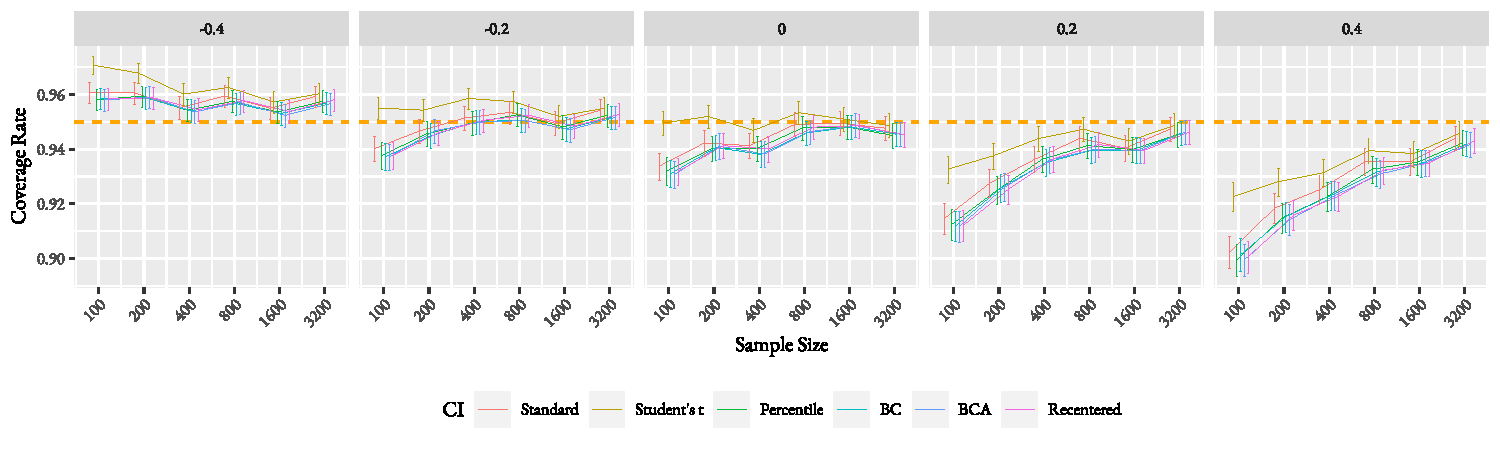
\includegraphics[width=\textwidth]{figures/alt_plot_norm_mu_1}
  \caption{Empirical coverage rates of different 95\% block bootstrap CIs for
    the marginal mean $\mu$ of an AR(1) process with a marginal standard 
    normal distribution with AR coefficient
    $\phi \in \{-0.4, 0.2, 0, 0.2, 0.4\}$ and series length
    $n \in \{100, 200, 400, 800, 1600, 3200\}$ based on 10,000 replicates. The
    error bars represent 95\% CIs of the real coverage rates.}
  \label{fig:mu}
\end{figure}

We find that this format
is a little
cluttered to make comparisons, so we have elected to remain with the original 
format.



\begin{comment}
3. The Appendix should be moved to the main text? Assessing the performance of 
various CI formulations for non-normal error is of central interest.
\end{comment} 

You are correct. To remedy this, the text highlighting the simulation study with 
an exponential marginal 
distribution from the Appendix has been moved to the Simulation Study 
section. 

\eds{I also added subsubsections (paragraphs) for the Normal and Exponential 
Marginal Distributions under Design and Results subsections.
Is it possible to put to make the [Simulation Study] Design and 
[Simulation Study] Results as two separate 
sections instead of placing each as subsections of the Simulation Study section,
or does the journal formatting prohibit this?  If you can change this, then the 
Normal and Exponential Marginal subsubsections can be updated to subsections
under the Simulation Study Design and Simulation Study Results sections.}  
\mc{addressed}


\jy{Left quote: `` (below the ESC key)}
\mc{addressed in reply and manuscript}

\begin{comment}
4. The authors might want to discuss in what circumstances “non-parametric” CI 
formulas would work better. It is a bit surprising that student’s t based 
formula works well under both normal and non-normal error structures.
\end{comment}

Thank you for the comment. We expect the CIs that 
are based on bootstrap 
``tables" to depend on the 
asymptotic distribution of the statistics, but we expect such CIs to 
have similar performance for different error structures. For example, under the 
Central
Limit Theorem, we expect the asymptotic distribution of the sample mean to be 
approximately 
normal for both marginal normal distributions and marginal exponential 
distributions. Therefore, we do not expect CIs that are not based on bootstrap
``tables" (Percentile, BC, BCA, Recentered Percentile CI) to perform better 
under
non-normal error structures. We have called attention to this in the Exponential
Marginal Distribution subsection of the Design section.

\eds{you will need to add more here.  This concerns the
(asymptotic) distribution of the statistics, not the underlying error 
structure.}
\mc{I changed it a bit... I'm not sure what to say for circumstances in which
“non-parametric” CI 
formulas would work better}


\begin{comment}
5. Page 3, 2nd line after “Standard Normal CI”: “p.168” does not seem to fit?
\end{comment}

Because of the bib style constraints for AJUR, we have removed page numbers in 
citations.

\subsection*{To Referee 2}

\begin{comment}
1. The authors say “....the standard CI is a table-based bootstrap…..”.  
What is meant by “table-based” here?  Is this just a reference to how critical 
values used to be listed in tables?  If that’s the case, I wouldn’t refer to 
this as a “table-based” interval. 
\end{comment}

Thank you for the comment.  This terminology was used because 
\citet{efron1993introduction} refers to such CIs as 
``confidence intervals based on 
bootstrap `tables'." We have replaced all instances of the phrase 
``table-based bootstrap CIs" to ``confidence intervals based on bootstrap 
`tables'" for the sake of clarity.

%The standard CI is classified by \citet{efron1993introduction} 
%as a confidence interval based on bootstrap ``tables".
%Like the standard normal interval, the
%Student's $t$ CI is classified by \citet{efron1993introduction} 
%as a confidence interval based on bootstrap ``tables".


\begin{comment}
2. Just a comment: The recentered percentile CI proposed here is an interesting 
interval to study. 
\end{comment}

We agree. We have added a comment in the Discussion underlining this CI's
potential for future investigations.

\begin{comment}
3. The sections are numbered, which makes it awkward when the authors refer back 
to a section.  For instance, they refer to “...procedures described in Block 
Bootstrap CIS.”  This would be easier to refer to if the sections were numbered.  
(Is this a journal style choice?  If so, then you can ignore this comment.)
\end{comment}

This is a journal style choice.

\begin{comment}
4.  In Figure 1 (and all the other figures), the authors present confidence 
intervals for the real coverage rates.  The authors should specify what type of 
CI they are using here.  I assume the authors are using a Wald-type interval for 
this CI as this is for a proportion.  If that’s the case, it’s well known that 
the Wald-type interval has undercoverage when the true proportion is near 0 or 
1, which is the case in several of these scenarios, especially when phi is -0.4. 
\end{comment}

Thank you for pointing this out. We modified the Design section to include a 
specification of the interval type for the coverage rate, as well as an 
acknowledgement of its flaw.

\eds{I don't think this answers the question.  The reviewer is saying that 0.95 
is close to the boundary of 1, so the undercoverage observed intervals
(especially when phi -0.4) may be due, at least in part, to the flaws 
of the asymptotic Wald interval you are using. 
\@ Jun: do you think he should try exact Clopper-Pearson
intervals for at least a few cases of undercoverage to verify it is not the Wald
interval that is causing the undercoverage, then comment on this in at least the
reply (and possibly also in the main paper)?}
\mc{plot\_norm\_mu\_1\_cup.pdf (exact Clopper-Pearson) seems to have about the same 
widths for high 
proportions
(especially for phi = -0.4) as {plot\_norm\_mu\_1.pdf} (Wald-Type)}
\jy{I thought the CP interval is for binomial proportions. How was it
  done here?}
\mc{this is the interval for the coverage rate, which is a proportion}


We have also included a figure in the Results section which 
uses exact 
Clopper-Pearson CIs to verify that the choice of interval
for the binomial proportion did not cause undercoverage in this case.

%CIs for $\mu$ exhibit coverage rates quite close to 1 for $\phi = -0.4$, and
%as stated before, the Wald-type CI is known to have undercoverage in such 
%situations.
%Figure~\ref{fig:norm_mu_1_cp} shows the same coverage rates using exact 
%Clopper-Pearson intervals to verify that it is the choice of Wald interval
%does not cause undercoverage of the coverage rate. Indeed, the widths of the
%exact proportion CIs do not seem to differ heavily from the Wald-type CIs.



\jy{No  need to duplicate the figures if they are already in the paper.}
\mc{addressed}


\begin{comment}
5.  In all the figures, the y-axis is allowed to vary freely making it hard to 
compare one row directly to another.  I would suggest fixing the limits on the 
y-axis to make comparisons easier.  
\end{comment}

Thank you for the suggestion. However, because of the deterioration for $\phi$, 
we found it hard to fix the limits on 
the 
y-axis without hurting the visualization for the other rows. 
Figure~\ref{fig:alt_phi1} is provided as an 
example:  \eds{refer to the Figure label, and avoid using `below' and `above'
terminology with latex because the figures are not always positioned as we may
have intended.}
\mc{addressed}

\begin{figure}[tbp]
  \centering
  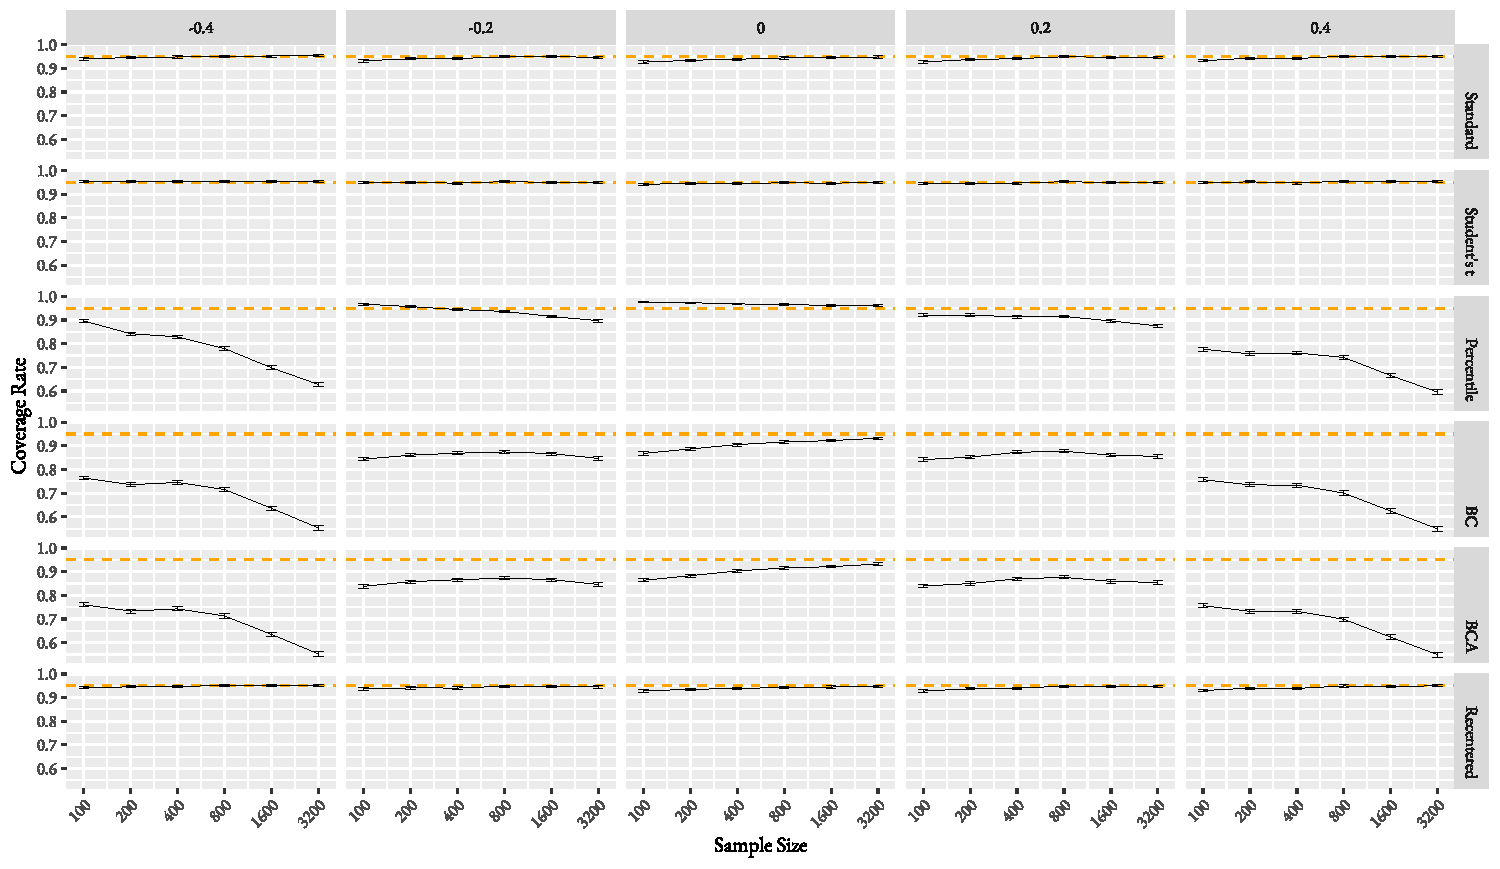
\includegraphics[width=\textwidth]{figures/alt2plot_norm_phi_1}
  \caption{Empirical coverage rates of different 95\% block bootstrap CIs for 
    the first-order autocorrelation coefficient $\phi$ of an AR(1) process with 
    a marginal standard normal distribution with 
    $\phi \in \{-0.4, 0.2, 0, 0.2, 0.4\}$ and series length
    $n \in \{100, 200, 400, 800, 1600, 3200\}$ based on 10,000 replicates of
    block bootstrap with $l = \lceil n^{1/3} \rceil$. The
    error bars represent 95\% CIs of the real coverage rates.}
  \label{fig:alt_phi1}
\end{figure}

\begin{comment}
6.  Is there a reason why the coverage for mu (in Figure 1) is better for 
negative autoregressive terms when compared with the positive autoregressive 
term? Can the authors give some intuition behind why that makes sense? 
\end{comment}

Thank you for this comment.
A possible explanation for this is that if a 
stationary series has a positive 
autocorrelation, the effective sample
size is decreased, whereas is a series has a negative autocorrelation, the
effective sample size is increased. Additionally, this seems to have a 
greater effect on the the estimation of the location parameter versus that
of the scale parameter or temporal dependence parameter. We have included a 
similar
comment at the end of the paragraph on estimation of 
$\mu$.

\begin{comment}
7.  The authors say “A smaller sample size is generally required to estimate a 
parameter for a sample with a negative phi versus a positive phi of the same 
magnitude.”  On a quick reading of this it sounds like the authors are 
recommending using a smaller sample size when phi is negative.  I believe what 
you are trying to say is that coverage rates are acceptable at smaller sample 
sizes when phi is negative versus when phi is positive (i.e. it takes larger 
sample sizes to get acceptable coverage when phi is positive).  Change this 
sentence to make it more clear. 
\end{comment}

Thank you for pointing this out. The original sentence has been reworded as you
suggested to make it more clear.

\begin{comment}
8.   In the Discussion section, the authors say “We know theoretically that the 
block bootstrap procedure will cover the parameter of a time series given an 
infinitely large sample.”  Essentially, you are stating that the estimator is 
consistent.  Is there a citation that you can point to that shows that this is 
true? 
\end{comment}

Thank you for drawing this to our attention. A citation \citep{calhoun2018} has
now been provided for that comment.

\eds{I only saw this citation in the abstract, not the discussion.  
Please remove this citation from the abstract and place in the discussion 
section where the sentence in question appears. In general,
try to avoid placing any citations in the abstract.}
\mc{addressed, sorry silly mistake}

\begin{comment}
9.   The authors studied coverage rates of the different intervals as a function 
of sample size, but they only looked at one choice for the number of blocks.  
Why did the authors choose to not also look at how the number of blocks affects 
the coverage rates?
\end{comment}

Thank you for the comment. We have now repeated the same simulation study with 
block size as an 
additional experimental factor. The optimal order of block size is 
$\lceil n^{1/3} \rceil$, so we tried the same simulations using 
$l = \lceil n^{1/3} \rceil$ and $l = \lceil 2n^{1/3} \rceil$. We have included
an Appendix detailing these results. 




\begin{comment}
10.   Why did the authors choose to only go as high as 0.4 (and as low as -0.4) 
for the autocorrelation parameter?  I would think that these correlations near 1 
(or -1) would be some of the more interesting cases to study, but they are 
completely ignored here.  Can the authors justify their choice to leave it out 
of this study?
\end{comment}

Thank you for the comment. We only
used serial dependences as strong as 0.4, because we only seek to 
establish the 
general trend as the strength of the autocorrelation 
increases, and how it varies depending on the sign of the autocorrelation and 
the parameter of interest. This justification has been added to the Design 
section.

\begin{comment}
11.    Last paragraph: The authors mention the “ABC and bootstrap-t intervals”.  
They do not give a citation for these intervals.   Add a citation. 
\end{comment}

We apologize for the omission. These intervals are discussed in 
\citep{efron1993introduction}. A citation is now provided in the last paragraph.

\begin{comment}
12.    The last line of the manuscript offers one line about the drawbacks of 
the block bootstrap almost as an afterthought.  I think a discussion of the 
drawbacks should be expanded and added to the introduction as this is an 
important point that isn’t mentioned at all until the literal last line. 
\end{comment}

Thank you for the comment. We have included a discussion of problems 
with block bootstrap in the introduction, while also highlighting its advantages
which motivated this investigation into their CI performance.


We are indebted to the reviewers for pointing out these vital discussion areas,
which have not only enriched the current paper but also charted a clear course
for our subsequent research endeavors.


\bibliographystyle{chicago}
\bibliography{citations}


\end{document}
